\setlength{\parskip}{\baselineskip}
\section{Related Work}

\begin{frame}
	\huge Related Work
\end{frame}

\begin{frame}
	\centering
	\huge{Software Frameworks}
	\vfill
	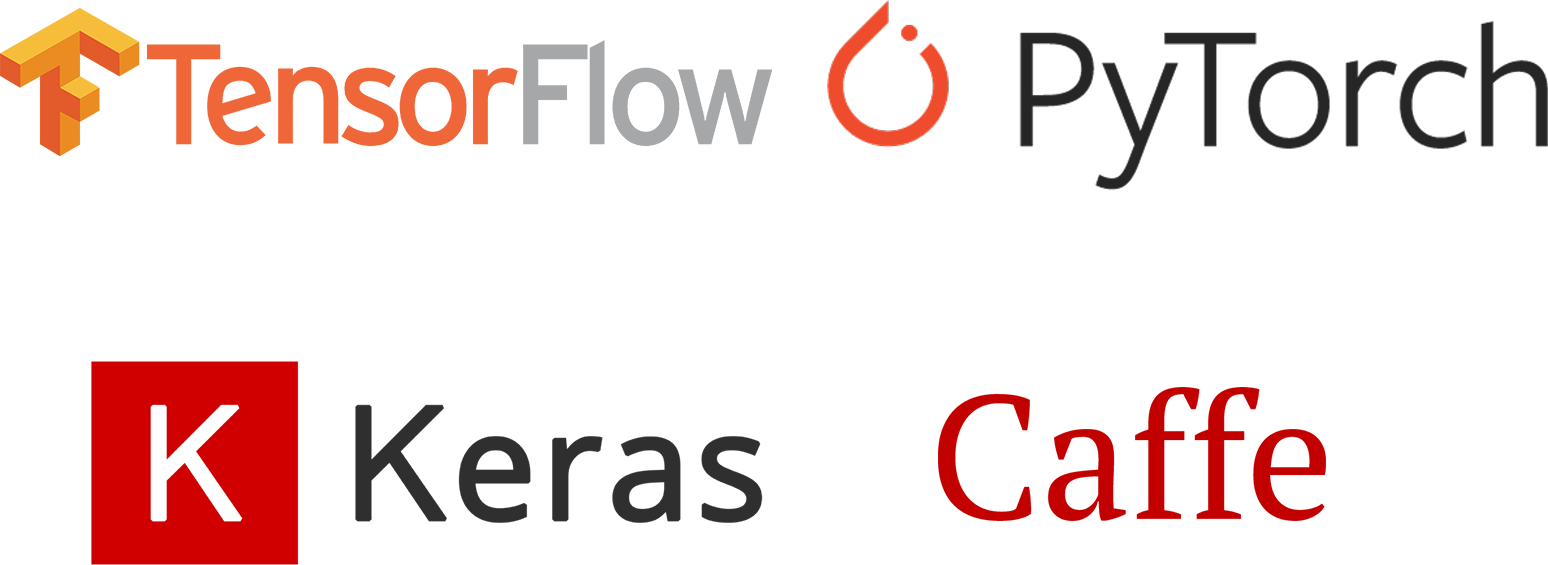
\includegraphics[width=0.95\textwidth]{../Images/CNNArchitectures/frameworks-logos.png}\\
\end{frame}

\begin{frame}{Software Frameworks: TensorFlow}
	\begin{minipage}{0.4\textwidth}
		\centering
		
\includegraphics[width=0.95\textwidth]{../Images/CNNArchitectures/tensorflow-logo.png}\\
	\end{minipage}%
	\begin{minipage}{0.6\textwidth}
		\begin{itemize}
			\item By Google
			\item Most popular
			\item Lower-level - Much coding - High Configurability
			\item Python, Javascript, C++, C\#, Java, Go \& Julia interfaces
			\item Targeted for production
			\item Static computation graph - Efficient but less flexible
			\item CPU, GPU \& TPU acceleration
			\item Server, Mobile \& Embedded platforms
		\end{itemize}
	\end{minipage}
\end{frame}

\begin{frame}{Software Frameworks: PyTorch}
	\begin{minipage}{0.4\textwidth}
		\centering
		
\includegraphics[width=0.95\textwidth]{../Images/CNNArchitectures/pytorch-logo.png}\\
	\end{minipage}%
	\begin{minipage}{0.6\textwidth}
		\begin{itemize}
			\item By Facebook
			\item Based on Torch
			\item CPU \& GPU acceleration
			\item Dynamically updated graph
			\item Targeted for prototyping \& research
			\item Contains many pre-trained models
		\end{itemize}
	\end{minipage}
\end{frame}

\begin{frame}{Software Frameworks: Keras}
	\begin{minipage}{0.4\textwidth}
		\centering
		
\includegraphics[width=0.95\textwidth]{../Images/CNNArchitectures/keras-logo.png}\\
	\end{minipage}%
	\begin{minipage}{0.6\textwidth}
		\begin{itemize}
			\item Higher-level
			\item Back-ends: TensorFlow, Theano \& CNTK
			\item Easy huge models - Less configurable
			\item Targeted for learning \& prototyping
		\end{itemize}
	\end{minipage}
\end{frame}

\begin{frame}{Software Frameworks: Caffe}
	\begin{minipage}{0.4\textwidth}
		\centering
		
\includegraphics[width=0.95\textwidth]{../Images/CNNArchitectures/caffe-logo.png}\\
	\end{minipage}%
	\begin{minipage}{0.6\textwidth}
		\begin{itemize}
			\item By Berkley, University of California
			\item Written in C++ - Python interface
			\item CPU \& GPU acceleration
			\item Not all Neural Networks supported
			\item Caffe2 merged with PyTorch
		\end{itemize}
	\end{minipage}
\end{frame}

\begin{frame}
	\centering
	\huge Hardware Frameworks
\end{frame}

\begin{frame}{Hardware Frameworks: Google TPU}
	\begin{minipage}{0.4\textwidth}
		\centering
		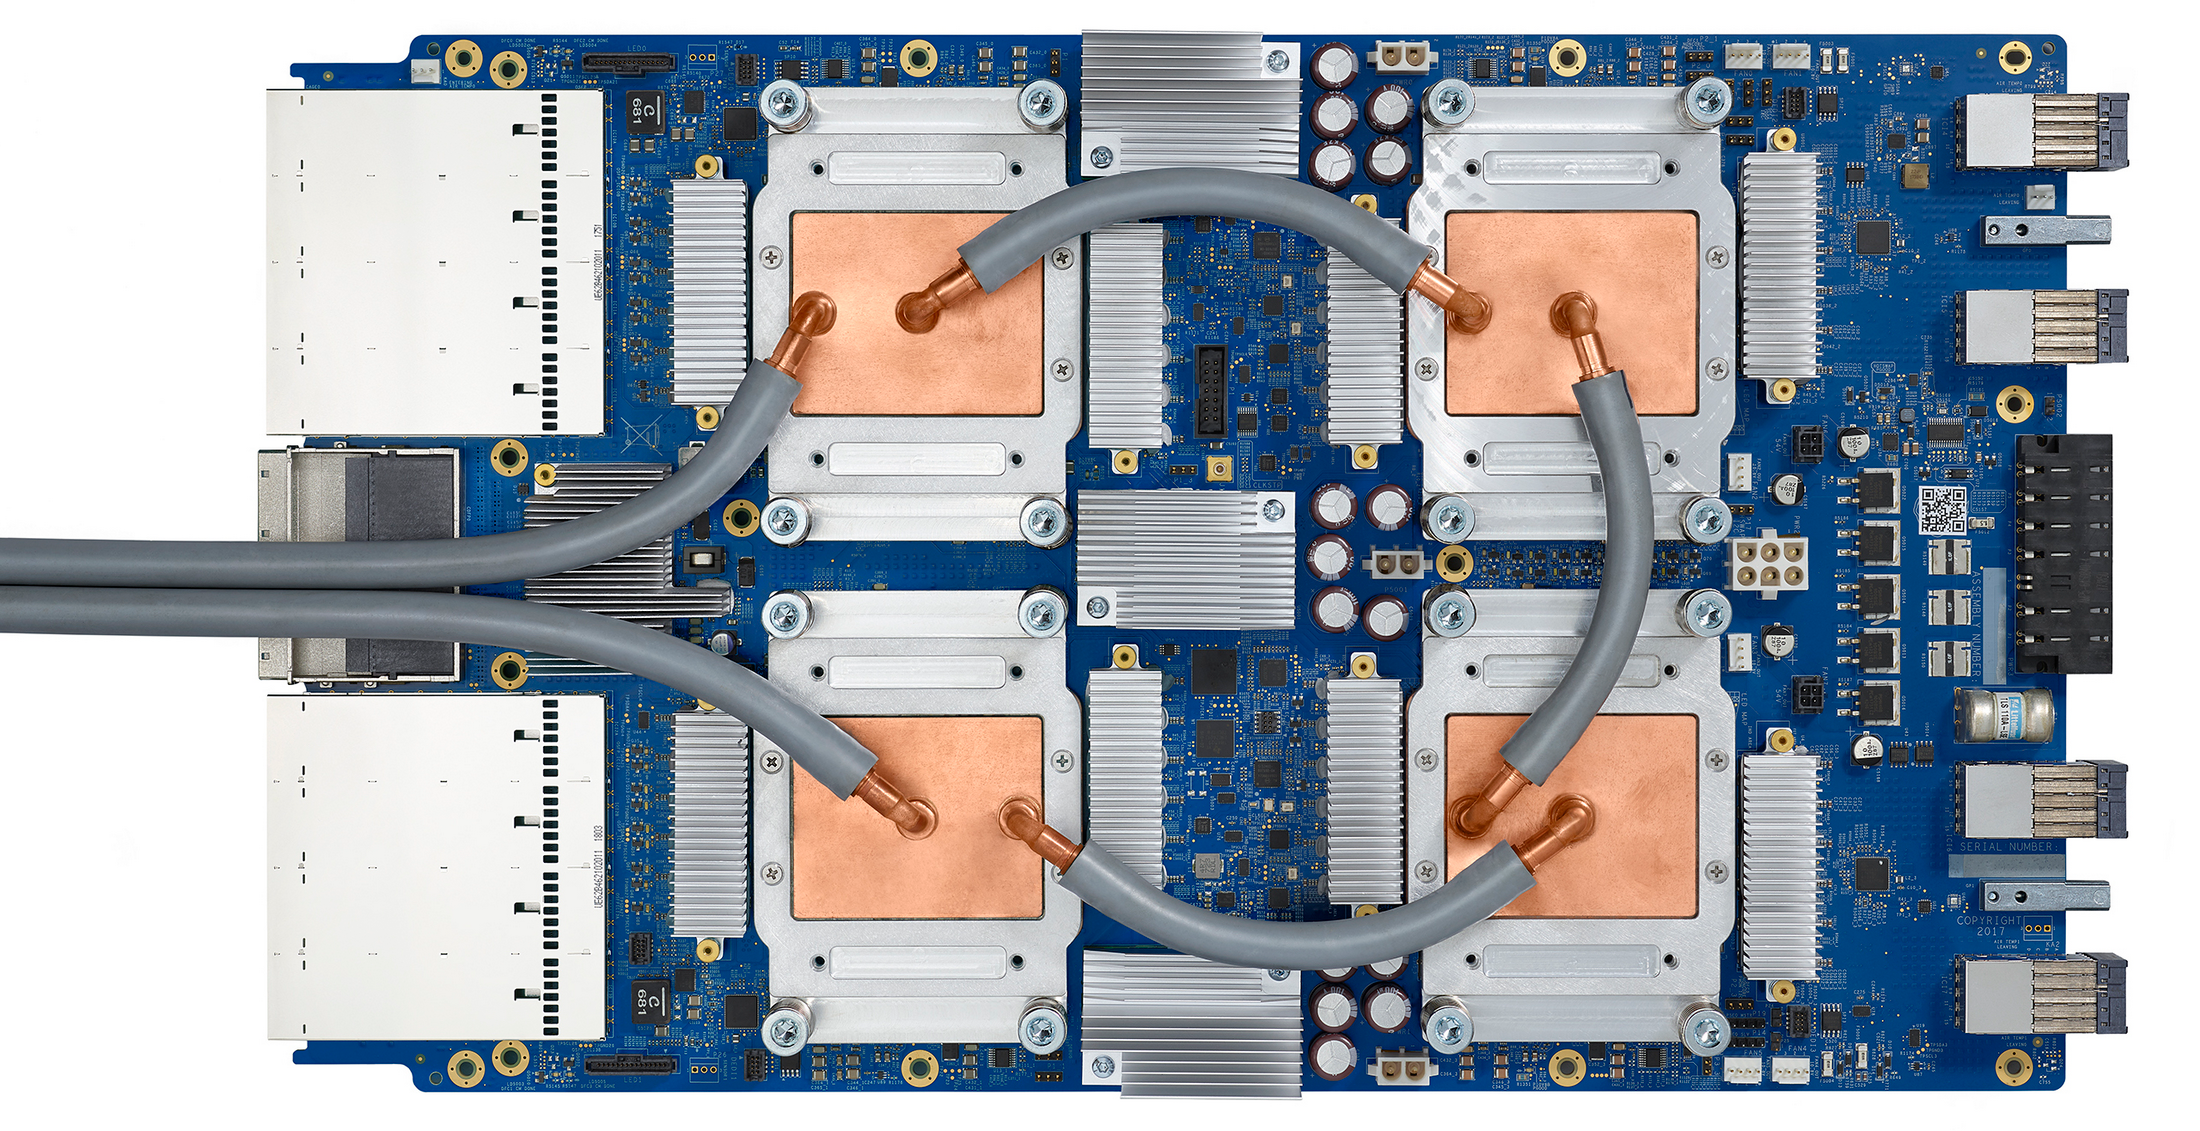
\includegraphics[width=0.9\textwidth]{../Images/Hardware/tpu-v3.png}\\
		Google TPU v3
	\end{minipage}%
	\begin{minipage}{0.6\textwidth}
		\begin{itemize}
			\item By Google since 2015
			\item Used with TensorFlow
			\item Accelerate 95\% of their AI needs
			\item Publicly available on Google Compute Engine since 2017
			\item Initially only inference \& 8-bit fixed-point
			\item 200x compared to Intel Haswell CPU
			\item 70x compared to NVIDIA K80 GPU
			\item Version 2 and above add training \& floating-point
		\end{itemize}
	\end{minipage}
\end{frame}

% \begin{frame}{Hardware Frameworks: Google TPU v1 Block Diagram}
% 	\centering
% 	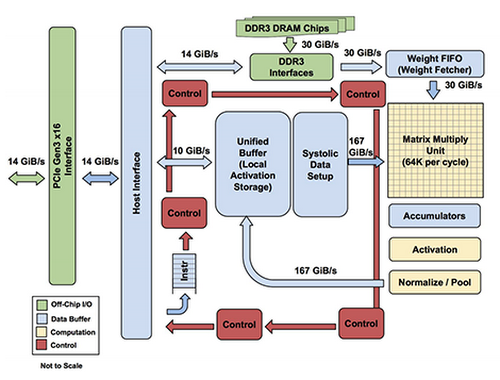
\includegraphics[width=0.45\textwidth]{../Images/Hardware/tpu-v1-block-diagram.png}
% 	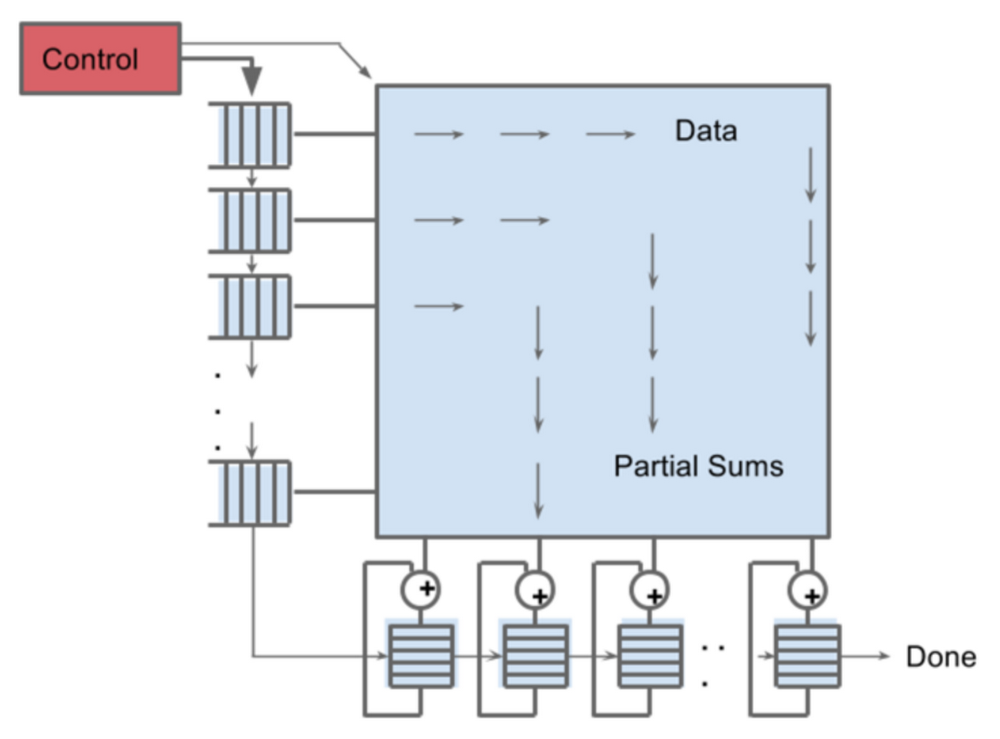
\includegraphics[width=0.45\textwidth]{../Images/Hardware/tpu-mxu.png}\\
% \end{frame}

\begin{frame}{Hardware Frameworks: Google TPU v1 Block Diagram}
	\begin{minipage}{0.4\textwidth}
		\centering
		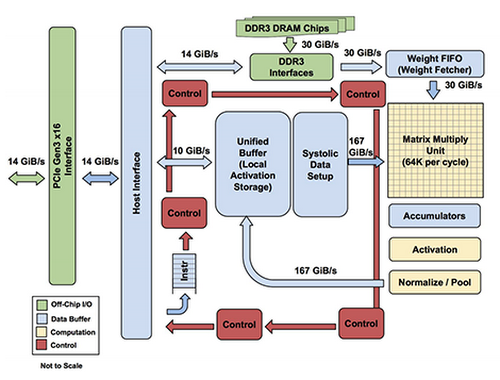
\includegraphics[width=0.95\textwidth]{../Images/Hardware/tpu-v1-block-diagram.png}\\
		TPU v1 Block Diagram
	\end{minipage}%
	\begin{minipage}{0.6\textwidth}
		\begin{itemize}
			\item Operate on matrices - GPUs operate on vectors
			\item 2x Matrix Multiplier Units (MXUs)
			\item MXU based on systolic arrays
			\item 16k MAC ops/cycle
			\item Up to 128GB HBM (TPU v3)
			\item 92 TOPS
		\end{itemize}
	\end{minipage}
\end{frame}

\begin{frame}{Hardware Frameworks: Google TPU v3 Pods}
	\begin{minipage}{0.7\textwidth}
		\centering
		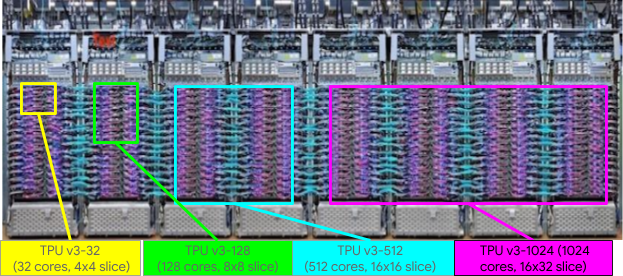
\includegraphics[width=0.9\textwidth]{../Images/Hardware/tpu-v3-pods.png}\\
	\end{minipage}%
	\begin{minipage}{0.3\textwidth}
		\begin{itemize}
			\item 2048 TPU Cores
			\item 32TB HBM
			\item 92 PFLOPS
			\item Suitable for very large models (weeks/months of training) - no custom operations
		\end{itemize}
	\end{minipage}
\end{frame}

\begin{frame}{FPGA Frameworks: Xilinx CHaiDNN}
	\begin{itemize}
		\item Released in February 2018 - Targeted for CNN inference
		\item 6-bit \& 8-bit fixed-point - variable through layers
		\item Similar to single-precision floating-point
		\item Dynamic fixed-point Quantization \& Xilinx Quantizer
		\item 128-1024 Double-Pumped DSPs - Up to 700MHz - URAM supported
		\item Unsupported layers added via Software
		\item Fully-Connected \& SoftMax layers implemented through Software
		\item Hardware \& Software layers run in parallel
		\item PetaLinux - Caffe framework
		\item DietCHai for smaller MPSoCs
	\end{itemize}
\end{frame}

\begin{frame}{FPGA Frameworks: Xilinx DPU}
	\begin{itemize}
		\item Released in February 2019 - Replaces CHaiDNN - Still in development
		\item Targeted for CNN inference - 8-bit fixed-point
		\item On-Chip memory utilized as buffer
		\item All layers are hardware accelerated
		\item Up to four DPU cores in a single DPU IP
		\item Double Data Rate / Double-Pumped DSPs
		\item 512-4096 operations per cycle per core
	\end{itemize}
\end{frame}

\begin{frame}{FPGA Frameworks: Xilinx DPU v1}
	\begin{minipage}{0.4\textwidth}
		\centering
		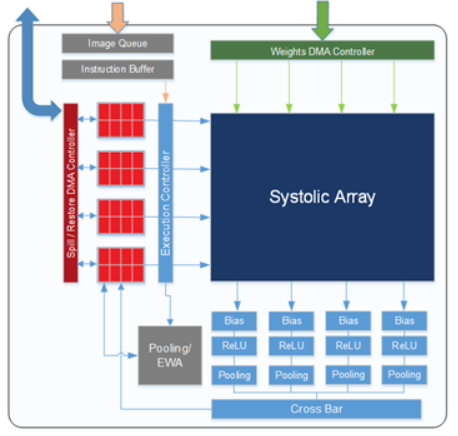
\includegraphics[width=0.95\textwidth]{../Images/Hardware/dpu-v1-architecture.png}\\
	\end{minipage}%
	\begin{minipage}{0.6\textwidth}
		\begin{itemize}
			\item 96x16 DSP Systolic Array
		\end{itemize}
	\end{minipage}
\end{frame}

\begin{frame}{FPGA Frameworks: Xilinx DPU v2}
	\begin{minipage}{0.4\textwidth}
		\centering
		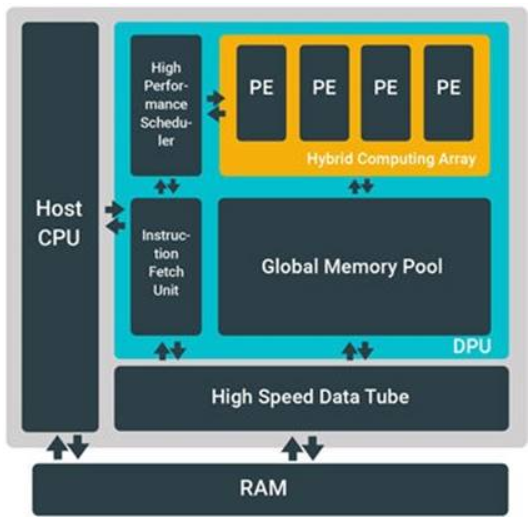
\includegraphics[width=0.95\textwidth]{../Images/Hardware/dpu-v2-architecture.png}\\
	\end{minipage}%
	\begin{minipage}{0.6\textwidth}
		\begin{itemize}
			\item Hybrid Computing Array
			\item Processing Elements - based on fine grained building blocks (multipliers, adders, accumulators)
			\item Deep Pipeline
		\end{itemize}
	\end{minipage}
\end{frame}

\begin{frame}{FPGA Frameworks: Xilinx DPU v3}
	\begin{minipage}{0.6\textwidth}
		\centering
		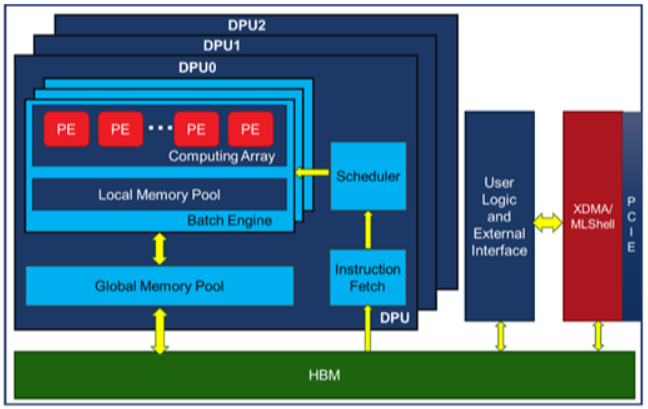
\includegraphics[width=0.9\textwidth]{../Images/Hardware/dpu-v3-architecture.png}\\
	\end{minipage}%
	\begin{minipage}{0.4\textwidth}
		\begin{itemize}
			\item Multiple Batch Engines
			\item Multiple DPU Cores
		\end{itemize}
	\end{minipage}
\end{frame}

\begin{frame}{FPGA Frameworks: Xilinx Vitis AI}
	\begin{minipage}{0.6\textwidth}
		\centering
		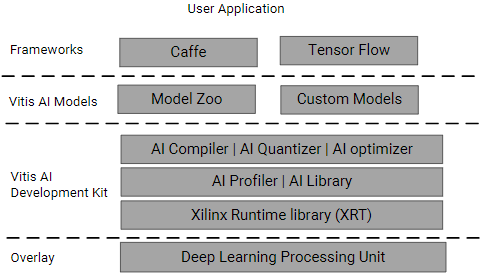
\includegraphics[width=0.9\textwidth]{../Images/Hardware/vitis-ai-stack.png}\\
	\end{minipage}%
	\begin{minipage}{0.4\textwidth}
		\begin{itemize}
			\item Released in December 2019
			\item High-level abstraction
			\item AI inference applications
			\item Based on Xilinx DPU
			\item Optimized IPs, tools \& libraries
			\item PetaLinux
			\item Instruction optimization - Vitis AI Compiler
			\item Vitis AI Quantizer - 8-bit fixed point parameters
		\end{itemize}
	\end{minipage}
\end{frame}

\begin{frame}{FPGA Frameworks: NVIDIA Deep Learning Accelerator (NVDLA)}
	\begin{minipage}{0.5\textwidth}
		\centering
		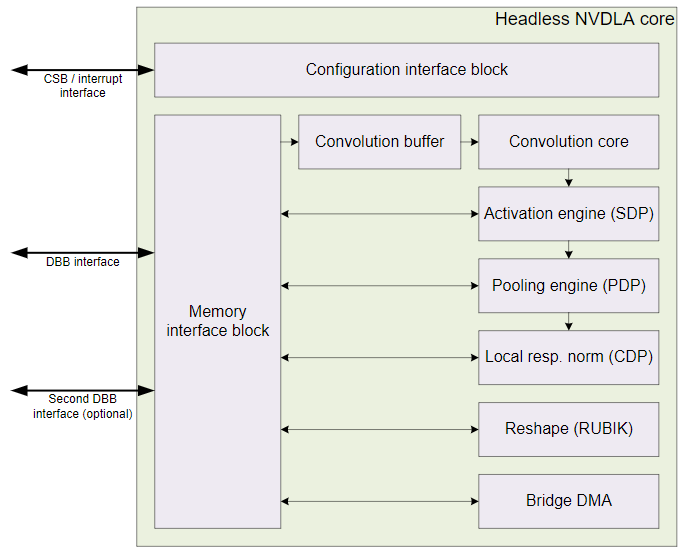
\includegraphics[width=0.9\textwidth]{../Images/Hardware/nvdla-hardware-architecture.png}\\
	\end{minipage}%
	\begin{minipage}{0.5\textwidth}
		\begin{itemize}
			\item Released in Q3 2017
			\item Free \& Open architecture
			\item Goal to standardize inference DL accelerator development
			\item Headless implementation: Manager is the main system processor
			\item Headed implementation: Manager is a companion microcontroller
			\item Modular \& Highly customizable
			\item Suitable for both FPGAs \& ASICs
		\end{itemize}
	\end{minipage}
\end{frame}

\begin{frame}{FPGA Frameworks: NVIDIA Deep Learning Accelerator (NVDLA)}
	\begin{minipage}{0.5\textwidth}
		\centering
		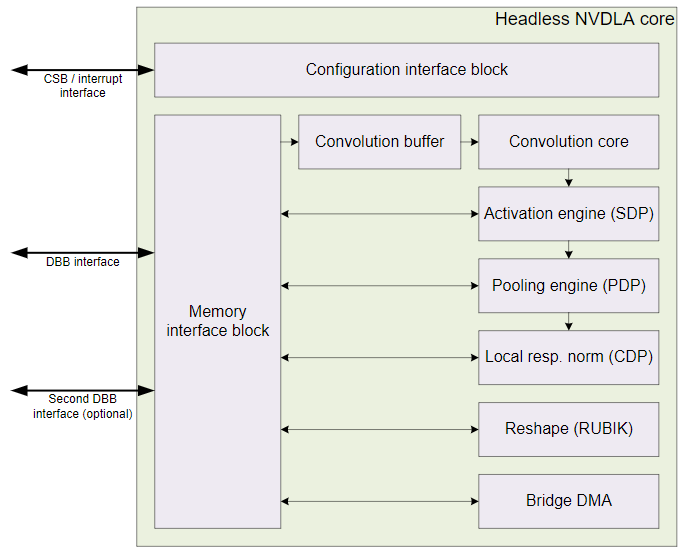
\includegraphics[width=0.9\textwidth]{../Images/Hardware/nvdla-hardware-architecture.png}\\
	\end{minipage}%
	\begin{minipage}{0.5\textwidth}
		\begin{itemize}
			\item Binary and 4-bit integer up to 64-bit floating-point
			\item Convolution core
			\item Single Data processor
			\item Planar Data processor
			\item Channel Data processor
			\item Data Reshape Engine
			\item Memory-to-Memory or Pass-Through
		\end{itemize}
	\end{minipage}
\end{frame}
